\documentclass[10pt,twocolumn]{article}

\usepackage[margin=0.75in]{geometry}
\usepackage{booktabs}
\usepackage{graphicx}
\usepackage{microtype}
\usepackage{times}
\usepackage{url}
\usepackage{xcolor}

\title{Pseudonymized but Linkable:\\
Cross-Document Re-identification Risks in LLM-Ready Sensitive Text Corpora}

\author{Anonymous Authors}
\date{}

\newcommand{\method}{LinkGuard}
\newcommand{\bench}{CrossDoc-PrivacyBench}

\begin{document}
\maketitle

\begin{abstract}
Sensitive text corpora are commonly de-identified one document at a time before retrieval, evaluation, or model adaptation.
We study a corpus-level failure mode for LLM-ready data: records with no direct identifiers can remain linkable through repeated quasi-identifiers such as role, region, schedule, institution type, family context, health context, and rare events.
We introduce \bench, a fully synthetic multi-document benchmark with 120 controlled personas, 480 documents, risk tiers, decoy auxiliary profiles, varied template families, and utility labels.
Direct redaction leaves auxiliary-profile matching unchanged at 0.708 top-1, while an off-the-shelf Presidio-style PII baseline remains highly matchable at 0.594.
We propose \method, a simple corpus-aware generalization procedure that estimates cross-document linkage risk and generalizes high-risk quasi-identifiers until a target anonymity set is reached.
At target $k=5$, \method{} reduces auxiliary top-1 accuracy to 0.042 while preserving issue classification and retrieval utility at 1.000; aggressive redaction reaches similar privacy but reduces issue accuracy to 0.350 and retrieval Recall@5 to 0.312.
A cached GPT-5.5 stress audit on 48 T2/T3 personas preserves this ordering, reinforcing that privacy evaluation for LLM-ready corpora should move beyond document-local PII removal and measure corpus-level linkage resistance.
\end{abstract}

\section{Introduction}
Organizations increasingly transform sensitive text into forms usable for retrieval-augmented generation, evaluation, fine-tuning, internal analytics, and data sharing.
The common operational unit is a document: remove names, emails, phone numbers, addresses, account numbers, and possibly other obvious personal identifiers from each record.
This document-local view is convenient, but it ignores a corpus-level threat.
If several documents belong to the same person or case, weak signals that appear harmless in isolation can become a stable signature when repeated across domains.

This paper asks a focused question: when sensitive corpora are pseudonymized or anonymized one document at a time, how much cross-document linkage risk remains?
We avoid real-person data and real re-identification attempts.
Instead, we build a controlled synthetic benchmark in which every persona, document, decoy, and utility label is generated by the experimenter.
This lets us evaluate attacks and defenses without collecting or exposing real sensitive text.

Our contributions are:
\begin{itemize}
    \item \textbf{Benchmark.} We introduce \bench, a synthetic cross-document privacy benchmark with 120 personas, 480 documents, four domains, risk tiers, utility labels, varied template families, and decoy auxiliary profiles.
    \item \textbf{Attack protocol.} We evaluate document linkage, auxiliary-profile matching, risk-tier stratification, and utility retention across multiple transformations.
    \item \textbf{Finding.} Direct redaction leaves strong auxiliary matching risk, document-local anonymization still misses high-risk combinations, and consistent pseudonyms act as stable linkage handles.
    \item \textbf{Defense.} We propose \method, a corpus-aware heuristic that generalizes quasi-identifiers according to corpus-level uniqueness, and show a privacy--utility tradeoff curve.
\end{itemize}

\section{Threat Model and Benchmark}
\paragraph{Threat model.}
A data holder has a multi-document sensitive text corpus and transforms it before indexing, sharing, or using it in foundation-model workflows.
The attacker sees the transformed corpus.
In the auxiliary-profile task, the attacker also sees a candidate set of synthetic profiles that simulate background knowledge.
The attacker's goals are to cluster documents belonging to the same synthetic persona and to match a cluster to the correct auxiliary profile.
All data in this study is synthetic; no real people, public profiles, social-media posts, patient records, legal records, or customer records are used.

\paragraph{Synthetic personas.}
\bench{} contains 120 personas.
Each persona has direct identifiers, quasi-identifiers, risk tier, and utility labels.
Quasi-identifiers include region, city, occupation, employer type, education, family structure, medical context, financial context, legal context, schedule pattern, affiliation, and rare event.
Each persona is assigned to one of three tiers:
T1 uses mostly direct PII with generic quasi-identifiers; T2 uses moderate quasi-identifiers; T3 uses high-linkage combinations.

\paragraph{Documents and utility labels.}
Each persona has four documents spanning healthcare, legal, financial support, and HR.
Documents include an issue label such as medication refill, benefits appeal, payment deferral, or schedule change.
Utility is measured by issue classification, task-oriented retrieval, and lightweight task-fact preservation.

\paragraph{Auxiliary profiles and decoys.}
For each persona, we construct a candidate set of one true synthetic profile and nine decoys.
Decoys share some attributes with the target, such as region, occupation family, or legal context, so matching is not a trivial exact-lookup task.

\section{Transformations}
We evaluate eight conditions.
C0 is the original synthetic document.
C1 performs direct redaction of names, email addresses, phone numbers, mailing addresses, and account IDs.
C1b applies Presidio-based PII detection plus local regex cleanup for synthetic account and address formats.
C2 uses stable pseudonyms across the corpus.
C3 resets pseudonym mappings per document.
C4 is a document-local anonymization proxy that generalizes direct identifiers and selected local spans without seeing neighboring documents.
C5 is \method.
C6 aggressively redacts most potentially identifying context.

\paragraph{\method.}
Document-local anonymizers ask whether a span is identifying inside one document.
\method{} asks whether a repeated detail makes a person distinguishable in the corpus.
For each persona group, it scores quasi-identifier fields by rarity, specificity, stability, and an approximate utility cost.
It then applies the lowest-cost privacy move until the transformed representation reaches a target anonymity set size.
Each field can move from exact value to semantic category, then to a generic suppression phrase.
The method is intentionally simple and should not be interpreted as a formal privacy guarantee.

\section{Attacks and Metrics}
\paragraph{Pairwise linkage and clustering.}
We compute quasi-identifier signatures and TF-IDF similarities over transformed documents.
Pairwise linkage is evaluated as same-person binary classification.
We also report fixed-$K$ clustering ARI, where $K$ is the true number of personas in the test split.
Threshold graph clustering is brittle outside stable-pseudonym settings, so we treat pairwise and auxiliary matching as the main privacy evidence.

\paragraph{Auxiliary matching.}
For each true persona cluster, an attacker ranks the ten synthetic auxiliary candidates.
We report top-1, top-3, and mean reciprocal rank.
Lower values are better for privacy.
We also report exact quasi-identifier recovery, a schema-aware profile-reconstruction scan over city, role, institution type, education, family, health, financial, legal, schedule, affiliation, and rare-event fields.
For a RAG-style exposure diagnostic, we issue exact synthetic auxiliary-profile queries against each transformed corpus and measure whether target-persona documents appear in top-$k$ retrieval.

\paragraph{Utility.}
We train local TF-IDF classifiers on original documents for domain and issue labels.
We also issue task queries such as domain plus issue phrase and measure whether documents with the same task label are retrieved in the top five.
We also score whether simple task-critical facts remain recoverable.
This utility evaluation is deliberately lightweight; it tests whether triage-relevant labels survive, not whether every downstream task is preserved.

\section{Results}
Table~\ref{tab:paper_main_results} reports the main local sweep over 96 held-out personas.
Direct redaction leaves auxiliary matching unchanged relative to original documents.
This supports the central failure mode: removing direct identifiers is insufficient when repeated quasi-identifiers remain.
The Presidio baseline removes direct PII through an off-the-shelf analyzer, but still leaves high auxiliary matching risk at 0.594 top-1 because the repeated quasi-identifiers remain.
The document-local proxy reduces some visible specificity, but auxiliary matching remains high.
Consistent pseudonymization yields pairwise linkage F1 of 0.979, showing that stable handles can make cross-document linkage almost trivial.
Exact quasi-identifier recovery tells the same story: direct redaction leaves exact recovery at 0.395, Presidio leaves 0.332, and the document-local proxy leaves 0.304.
Bootstrap 95\% confidence intervals over held-out personas keep the main auxiliary-matching contrast separated: direct redaction 0.708 [0.615, 0.802], Presidio 0.594 [0.490, 0.698], and \method{} 0.042 [0.010, 0.083].
Risk-tier stratification confirms that the benchmark varies linkage difficulty: under direct redaction Aux@1 rises from 0.156 on T1 to 0.969 on T2 and 1.000 on T3, while \method{} lowers the corresponding rates to 0.031, 0.000, and 0.094.
A no-API robustness sweep over three independently generated corpus seeds preserves this ordering: direct redaction, Presidio, and the document-local proxy have mean auxiliary top-1 of 0.719, 0.628, and 0.663, while \method{} averages 0.045 with retrieval Recall@5 at 1.000.
A noisy-style synthetic rerendering lowers mean template similarity to 0.306 and preserves the ordering: direct/Presidio/document-local Aux@1 0.656/0.562/0.594, \method{} 0.042 with issue/Ret@5 1.000, and aggressive redaction issue/Ret@5 0.473/0.635.
Single-signal ablations of direct-redacted documents indicate that role/institution and location are the largest local drivers, reducing auxiliary top-1 to 0.500 and 0.521 when removed.
Expanding the auxiliary candidate pool from 10 to 50 candidates preserves the ordering: direct redaction remains at 0.635 top-1, the document-local proxy at 0.500, and \method{} at 0.000 against a 0.020 chance baseline.
Across word, character, hybrid TF-IDF, and field-weighted auxiliary matchers, direct redaction remains at 0.510--0.979 top-1 and the document-local proxy at 0.479--0.979, while \method{} remains lower at 0.031--0.240.
The field-weighted attacker is strongest because it scans exact and generalized quasi-identifier fields; it exposes residual structured-context risk under \method{}, but still leaves a large gap from document-local baselines.
In the RAG exposure diagnostic, exact profile queries against high-linkage T3 personas retrieve at least one target document in the top five for every direct-redacted, Presidio-redacted, and document-local corpus (Hit@5 1.000), and retrieve multiple target documents in the top ten for every such persona (Multi@10 1.000); \method{} reduces T3 Hit@5 to 0.312 and Multi@10 to 0.000.
A deterministic top-5 RAG context-recovery scan on T3 profiles recovers 9.781 exact fields under direct redaction and 7.844 exact / 9.469 coarse fields under document-local anonymization, but only 0.000 exact / 0.438 coarse fields under \method{}.

\begin{table}[t]
\centering
\scriptsize
\setlength{\tabcolsep}{3pt}
\caption{Sprint benchmark results. Lower is better for Pair F1, Aux@1, Exact quasi-identifier recovery, and Edit; higher is better for Issue, Ret@5, and Facts.}
\label{tab:paper_main_results}
\begin{tabular}{lrrrrrrr}
\toprule
Cond. & Pair & Aux@1 & Exact & Issue & Ret@5 & Facts & Edit \\
\midrule
C0 Orig & 0.963 & 0.708 & 0.395 & 1.000 & 1.000 & 0.682 & 0.000 \\
C1 Redact & 0.214 & 0.708 & 0.395 & 1.000 & 1.000 & 0.682 & 0.246 \\
C1b Presidio & 0.142 & 0.594 & 0.332 & 1.000 & 1.000 & 0.682 & 0.348 \\
C2 Stable & 0.979 & 0.427 & 0.273 & 1.000 & 1.000 & 0.679 & 0.299 \\
C3 PerDoc & 0.148 & 0.427 & 0.273 & 1.000 & 1.000 & 0.679 & 0.315 \\
C4 Local & 0.155 & 0.604 & 0.304 & 1.000 & 1.000 & 0.682 & 0.288 \\
C5 LG & 0.019 & 0.042 & 0.000 & 1.000 & 1.000 & 0.695 & 0.535 \\
C6 Agg & 0.016 & 0.052 & 0.000 & 0.350 & 0.312 & 0.389 & 0.681 \\
\bottomrule
\end{tabular}
\end{table}


\paragraph{Corpus-aware generalization.}
\method{} reduces auxiliary matching to 0.042 while preserving issue accuracy and retrieval Recall@5 at 1.000.
Aggressive redaction reaches a similar privacy level, but issue accuracy falls to 0.350 and retrieval Recall@5 falls to 0.312.
In a stricter body-only utility stress test that removes subject and contact scaffolding, \method{} scores 0.880, close to direct redaction at 0.870, while aggressive redaction falls to 0.438.
Thus, in this synthetic sprint, \method{} occupies a better privacy--utility point than blanket redaction.
Figure~\ref{fig:frontier} visualizes this tradeoff.

\begin{figure}[t]
    \centering
    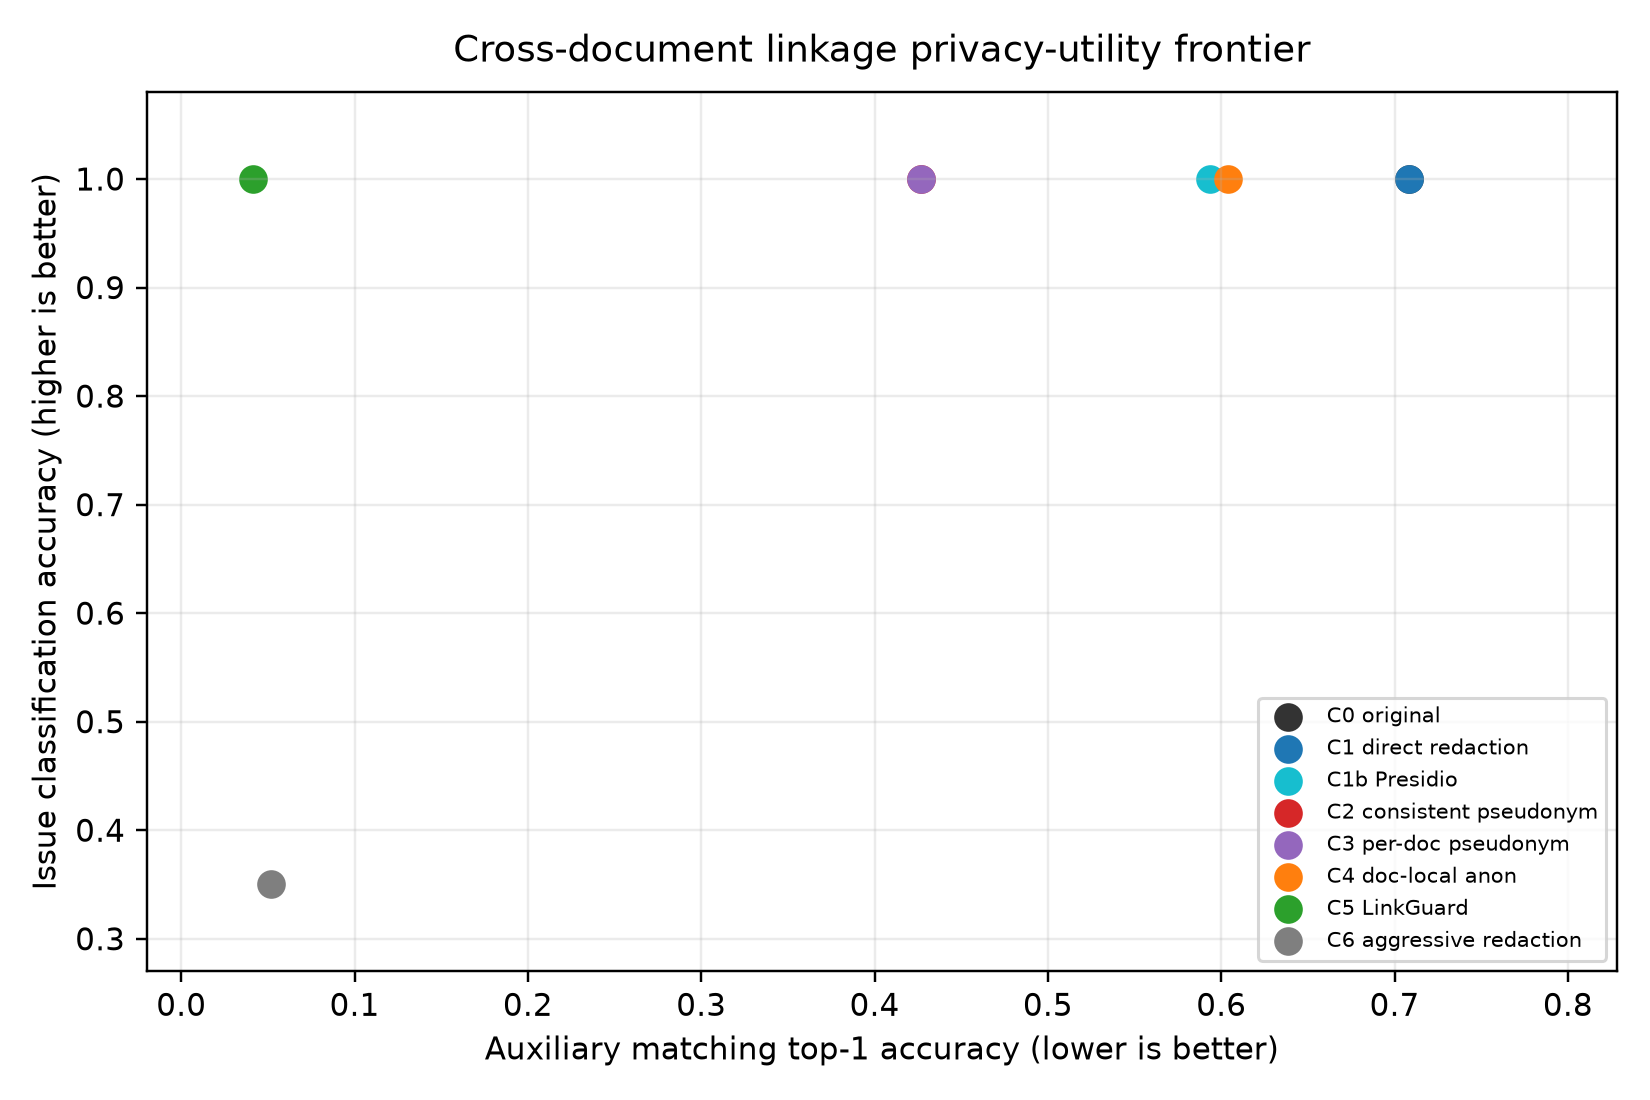
\includegraphics[width=\linewidth]{figures/privacy_utility.png}
    \caption{Privacy--utility frontier. Lower auxiliary matching is better for privacy; higher issue accuracy is better for utility.}
    \label{fig:frontier}
\end{figure}

\paragraph{Sensitivity to target $k$.}
Table~\ref{tab:linkguard_sensitivity} shows that most of the privacy gain appears once \method{} moves from direct redaction ($k=1$) to target $k=2$.
Auxiliary top-1 drops from 0.708 to 0.062, while higher targets provide diminishing attack reduction with modest additional edit cost.
Exact quasi-identifier recovery also falls from 0.395 at $k=1$ to 0.007 at $k=2$ and 0.000 at $k=5$.
Under the field-weighted stress attacker, top-1 falls from 0.979 at $k=1$ to 0.240 at $k=5$ and 0.104 at $k=20$, suggesting that corpus-aware generalization can be treated as a controllable risk budget rather than a single fixed transformation.

\begin{table}[t]
\centering
\scriptsize
\setlength{\tabcolsep}{3pt}
\caption{LinkGuard sensitivity to target k.}
\label{tab:linkguard_sensitivity}
\begin{tabular}{lrrrrrrrr}
\toprule
k & Min k & Edit & Pair & Aux@1 & Field@1 & Exact & Issue & Ret@5 \\
\midrule
1.000 & 1.000 & 0.246 & 0.214 & 0.708 & 0.979 & 0.395 & 1.000 & 1.000 \\
2.000 & 2.000 & 0.521 & 0.036 & 0.062 & 0.354 & 0.007 & 1.000 & 1.000 \\
3.000 & 3.000 & 0.528 & 0.029 & 0.052 & 0.333 & 0.004 & 1.000 & 1.000 \\
5.000 & 5.000 & 0.535 & 0.019 & 0.042 & 0.240 & 0.000 & 1.000 & 1.000 \\
8.000 & 8.000 & 0.538 & 0.017 & 0.042 & 0.167 & 0.000 & 1.000 & 1.000 \\
12.000 & 12.000 & 0.539 & 0.017 & 0.042 & 0.125 & 0.000 & 1.000 & 1.000 \\
20.000 & 20.000 & 0.544 & 0.017 & 0.042 & 0.104 & 0.000 & 1.000 & 1.000 \\
\bottomrule
\end{tabular}
\end{table}


\begin{figure}[t]
    \centering
    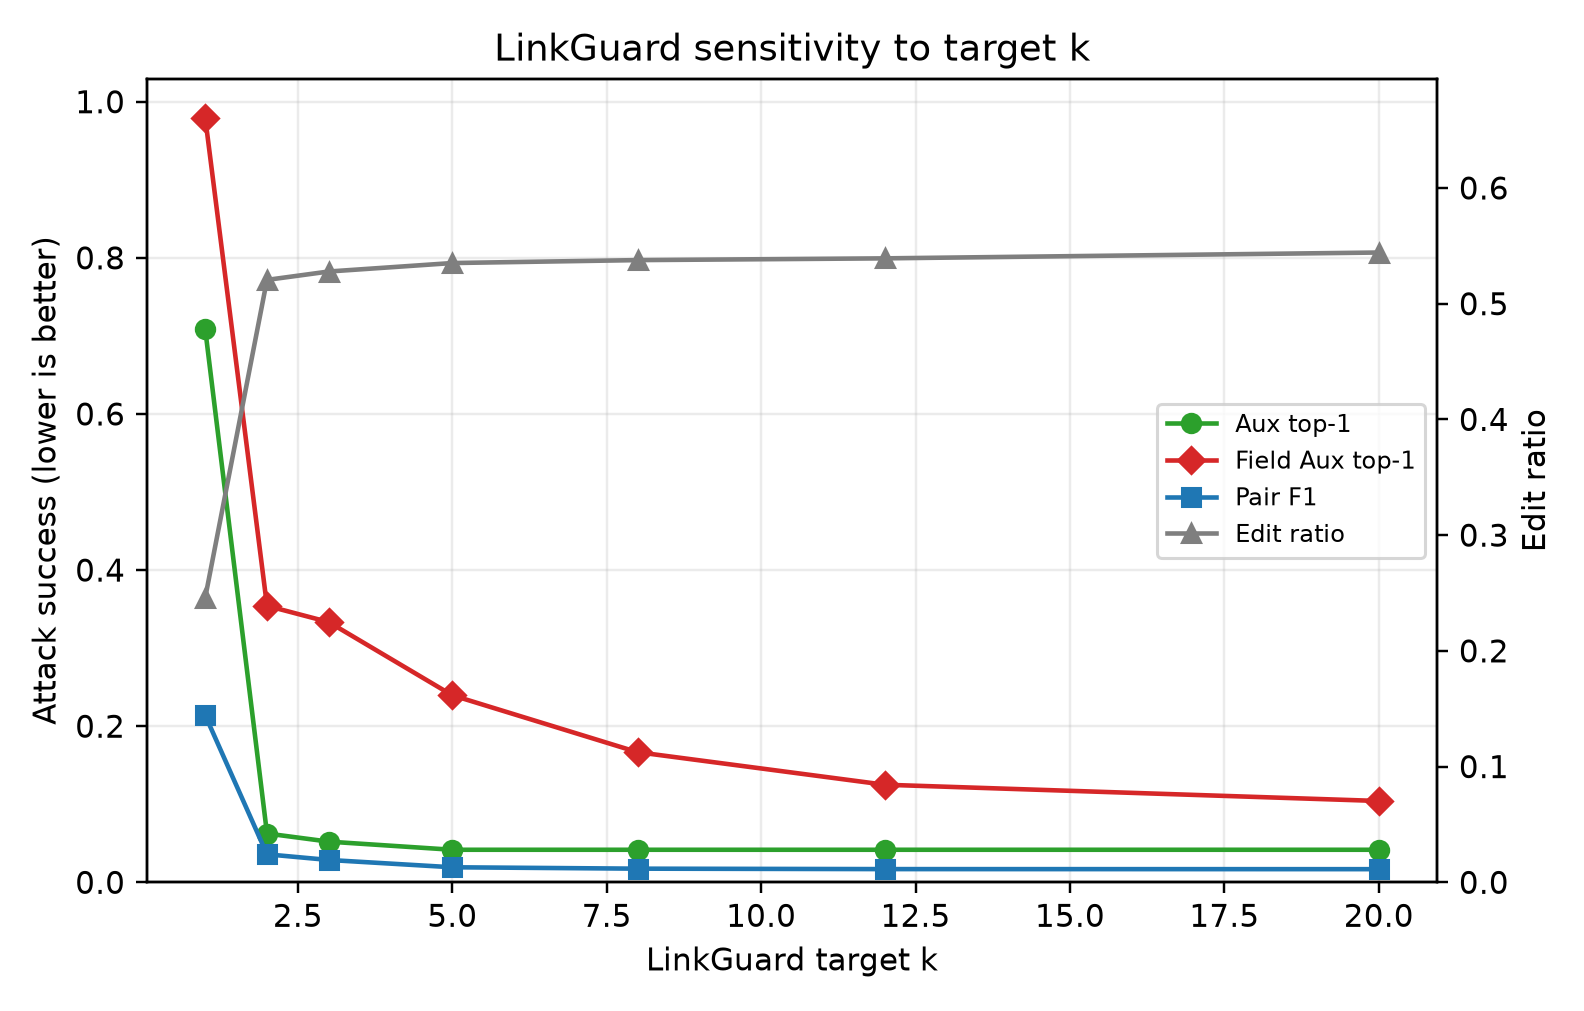
\includegraphics[width=\linewidth]{figures/linkguard_sensitivity.png}
    \caption{\method{} sensitivity to target $k$. The main auxiliary matcher drops sharply by $k=2$, while the field-weighted stress attacker continues to improve at larger $k$.}
    \label{fig:sensitivity}
\end{figure}

\paragraph{GPT-5.5 API stress audit.}
We also ran a time-stamped GPT-5.5 auxiliary-matching audit on 48 T2/T3 personas, using synthetic data only, capped calls, cached responses, and \texttt{store=false}.
Because API model behavior can change, we treat this as corroborating stress evidence rather than the main reproducible result.
Direct redaction, Presidio redaction, and the document-local proxy remain highly matchable at 1.000, 0.979, and 1.000 top-1.
\method{} lowers top-1 to 0.438, with high model-reported uncertainty, while aggressive redaction is 0.333.
A separate 24-person GPT-5.5 document-local anonymization baseline also remains fully matchable at 1.000 top-1, compared with 0.333 for \method{} on the same subset.
An additional 24-case GPT-5.5 evidence-extraction audit finds that direct-redaction successful matches cite location in 1.000 and role in 0.750 of cases, while \method{} residual matches cite role, location, and institution at 0.000 and are uncertain in 0.875.

\begin{table}[t]
\centering
\small
\setlength{\tabcolsep}{3pt}
\caption{GPT-5.5 instruction-following auxiliary matching audit on 48 T2/T3 synthetic personas. Unc. is the model-reported uncertainty rate.}
\label{tab:gpt55_aux_audit}
\begin{tabular}{lrrrrrr}
\toprule
Cond. & n & Aux@1 & Aux@3 & T2@1 & T3@1 & Unc. \\
\midrule
C1 Redact & 48 & 1.00 & 1.00 & 1.00 & 1.00 & 0.02 \\
C1b Presidio & 48 & 0.98 & 1.00 & 0.96 & 1.00 & 0.12 \\
C4 Local & 48 & 1.00 & 1.00 & 1.00 & 1.00 & 0.08 \\
C5 LG & 48 & 0.44 & 0.71 & 0.42 & 0.46 & 0.92 \\
C6 Agg & 48 & 0.33 & 0.67 & 0.42 & 0.25 & 0.79 \\
\bottomrule
\end{tabular}
\end{table}


\section{Related Work}
Classic work on $k$-anonymity argues that released records can remain re-identifiable through combinations of quasi-identifiers, motivating generalization and suppression \cite{sweeney2002}.
Sparse-data de-anonymization attacks show that seemingly weak auxiliary knowledge can identify records in high-dimensional datasets \cite{narayanan2008}.
Text anonymization benchmarks such as TAB evaluate privacy-oriented span masking in text \cite{pilan2022tab}, and RAT-Bench recently reframes text anonymization around re-identification risk from direct and indirect identifiers \cite{krco2026ratbench}.
Recent work on LLM privacy inference shows that language models can infer personal attributes from text beyond direct memorization \cite{staab2024beyond}.
RAG privacy work shows that retrieval databases themselves can leak sensitive records through generated outputs \cite{zeng2024ragprivacy}.
Presidio provides widely used open-source tools for PII analysis and anonymization \cite{presidio}.
Our contribution is complementary: we focus on cross-document linkage after document-level transformations, where repeated corpus-level quasi-identifiers can survive otherwise reasonable LLM-ready anonymization workflows.

\section{Limitations and Ethics}
This work uses synthetic data only.
That is necessary for controlled, reproducible, non-harmful evaluation, but it limits external validity.
The corpus uses controlled template families, and real corpora may contain different stylistic, temporal, and institutional distributions.
Our local attacks are simple, and the GPT-5.5 audit is a time-stamped API stress test rather than a stable benchmark.
\method{} is a heuristic and does not provide a formal anonymity guarantee.
Finally, utility is measured through issue labels and lightweight fact checks; stronger downstream utility evaluations are needed before operational deployment.

The benchmark is intended for defensive auditing.
We do not collect, process, or attempt to re-identify real people.
Auxiliary profiles are synthetic and generated from the same controlled schema.
Any extension to real data would require authorization, data-minimization safeguards, and ethical review.

\section{Conclusion}
Document-local PII removal is not enough for LLM-ready sensitive corpora.
In a multi-document setting, repeated quasi-identifiers can link records and support auxiliary-profile matching even after direct identifiers are removed.
Our synthetic benchmark and initial results show that privacy evaluation should include corpus-level linkage resistance.
They also suggest that simple corpus-aware generalization can improve the privacy--utility frontier relative to both document-local anonymization and blanket redaction.

\bibliographystyle{plain}
\begin{thebibliography}{11}

\bibitem{krco2026ratbench}
Nata{\v{s}}a Kr{\v{c}}o, Zexi Yao, Matthieu Meeus, and Yves-Alexandre de Montjoye.
\newblock RAT-Bench: A comprehensive benchmark for text anonymization.
\newblock \emph{arXiv:2602.12806}, 2026.

\bibitem{narayanan2008}
Arvind Narayanan and Vitaly Shmatikov.
\newblock Robust de-anonymization of large sparse datasets.
\newblock In \emph{IEEE Symposium on Security and Privacy}, 2008.

\bibitem{pilan2022tab}
Ildikó Pilán, Pierre Lison, Lilja {\O}vrelid, Anthi Papadopoulou, David S{\'a}nchez, and Montserrat Batet.
\newblock The Text Anonymization Benchmark (TAB): A dedicated corpus and evaluation framework for text anonymization.
\newblock \emph{Computational Linguistics}, 2022.

\bibitem{presidio}
Microsoft.
\newblock Presidio: Data protection and de-identification SDK.
\newblock \url{https://microsoft.github.io/presidio/}.

\bibitem{staab2024beyond}
Robin Staab, Mark Vero, Mislav Balunovi{\'c}, and Martin Vechev.
\newblock Beyond memorization: Violating privacy via inference with large language models.
\newblock In \emph{International Conference on Learning Representations}, 2024.

\bibitem{sweeney2002}
Latanya Sweeney.
\newblock Achieving $k$-anonymity privacy protection using generalization and suppression.
\newblock \emph{International Journal of Uncertainty, Fuzziness and Knowledge-Based Systems}, 2002.

\bibitem{zeng2024ragprivacy}
Shenglai Zeng et al.
\newblock The good and the bad: Exploring privacy issues in retrieval-augmented generation.
\newblock \emph{arXiv:2402.16893}, 2024.

\end{thebibliography}

\end{document}
